\section{系統架構與設計}

\subsection{整體架構}

圖~\ref{fig:architecture} 整理了程式中幾個主要部分。Application 負責建立與保留各個 Window；PaintWindow 將操作介面、選單、快捷鍵與 Document 組合起來。使用者完成一次繪圖後，Canvas 會把結果交給 Document，Document 再修改 Scene。Renderer 只讀取 Scene 的內容，依物件種類選擇圖形或文字的繪製方式。

\begin{figure}[H]
    \centering
    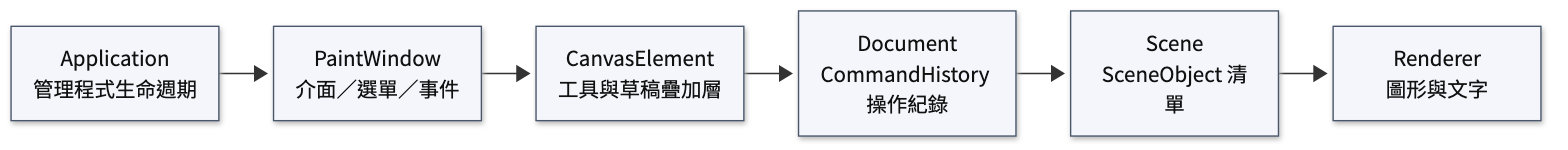
\includegraphics[width=.96\textwidth]{docs/figures/architecture.png}
    \caption{繪圖程式的整體架構}
    \label{fig:architecture}
\end{figure}

\subsection{Application 與 Window}

FreeGLUT 本身可以建立多個視窗，但不會替 C++ 程式管理物件生命週期。我因此讓 Application 管理所有 Window，新的 Paint Window、Input Dialog、Confirm Dialog 與圖片輸出用視窗都從同一個入口建立。視窗收到關閉要求後先標記狀態，之後再由 idle callback 移除，避免 callback 還在執行時物件就被釋放。

另一個問題是 FreeGLUT 只接受 C-style callback，不能直接綁定某個 Window instance。程式建立一張以 GLUT window ID 為 key 的查找表；static callback 先取得目前視窗 ID，再找回真正要處理事件的 Window。程式碼~\ref{lst:window-lookup} 是這段轉接的核心，完整流程則畫在圖~\ref{fig:callback-routing}。多視窗與 Modal Dialog 的生命週期放在附錄~\ref{app:gui}。

Hierarchical Menu 也有類似限制：FreeGLUT 的 menu callback 只會傳回整數 ID。Menu class 因此替每個選項記錄 ID 與動作的對照，收到 callback 後先找回項目，再執行綁定的功能。這讓 PaintWindow 可以用一般 lambda 設定選單行為，不必把所有功能塞進同一個 switch。

\begin{lstlisting}[caption={由 GLUT window ID 找回 C++ Window instance},label={lst:window-lookup}]
Window* Window::currentWindow() {
    const int id = glutGetWindow();
    auto it = windows.find(id);
    if (it != windows.end()) {
        return it->second;
    }
    return nullptr;
}
\end{lstlisting}

\begin{figure}[H]
    \centering
    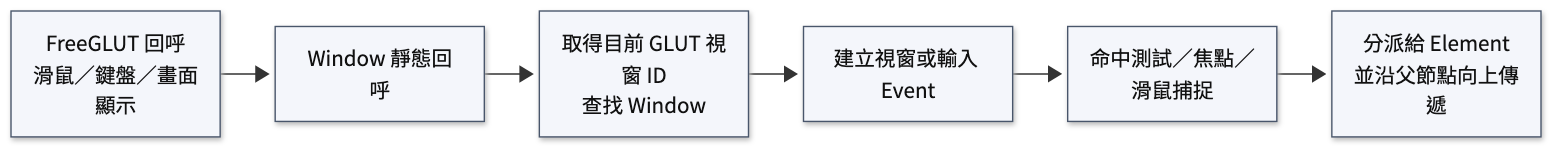
\includegraphics[width=.98\textwidth]{docs/figures/callback-routing.png}
    \caption{GLUT 回呼的路由流程}
    \label{fig:callback-routing}
\end{figure}

\subsection{Document、Scene 與 Shape}

Document 記錄檔名、Canvas 尺寸、Scene 與 Command History，是繪圖內容修改的入口。Scene 依照繪製順序儲存 SceneObject，其中 ShapeObject 包含 Point、Line、Rectangle、Ellipse、Path 與 Polygon，TextObject 則記錄文字位置、UTF-8 字串與文字樣式。

這樣分層之後，Scene 不需要知道 UI，也不會直接呼叫 OpenGL。工具完成時只產生一個 SceneObject，再由 Document 建立 Command 修改 Scene。拖曳中的 draft 留在 tool overlay，所以尚未完成的圖形不會先進入 Scene，也不會多產生一筆 Undo 紀錄。

\subsection{Event 與 Input}

滑鼠事件進入 Window 後，程式會先從 Element tree 中找出游標所在的最深層元件；若某個元件已取得 mouse capture，就直接把事件送到該元件。Listener 執行完後，Input Event 會沿著 parent chain 向上傳遞，最後到達 Window。元件如果已經處理完事件，可以呼叫 \lstinline|stopPropagation()|，避免同一個輸入又被上層重複處理。圖~\ref{fig:event-propagation} 顯示這個過程。

\begin{figure}[H]
    \centering
    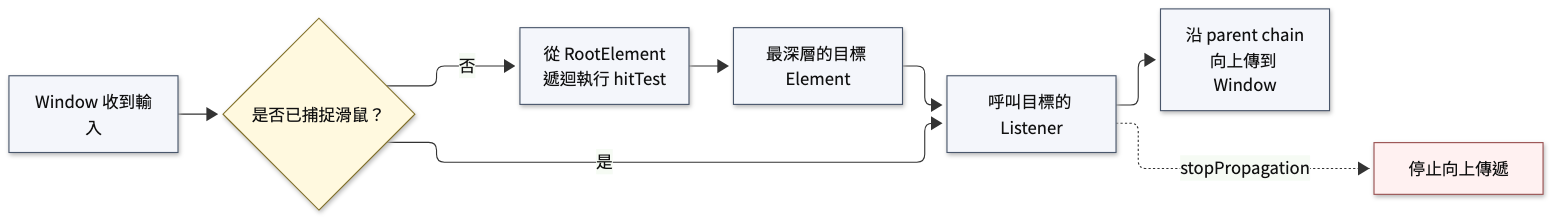
\includegraphics[width=.98\textwidth]{docs/figures/event-propagation.png}
    \caption{Event 目標選取與沿父節點向上傳遞的流程}
    \label{fig:event-propagation}
\end{figure}

每個輸入事件都會附帶當下的 keyboard 與 mouse state，因此工具在處理 Motion 時，可以同時判斷 Shift 是否按下以及 MouseLeft 是否仍在拖曳。ShortcutManager 若遇到多個可能的 KeyChord，會優先選擇按鍵數較多的組合，避免較短的快捷鍵先被觸發。

\subsection{Command History 與 Undo/Redo}
\label{sec:command-history}

加入、插入、移除物件與清空畫布都會建立可以復原的 Command。新的 Command 執行後會進入 undo stack，同時清空 redo stack；Undo 會執行反向操作，並把同一筆紀錄移到 redo stack，Redo 則再次執行它。除了兩個 stack 之外，每筆紀錄還記錄操作前後的 state ID，讓程式可以判斷目前內容是否回到上次儲存的狀態。圖~\ref{fig:command-history} 整理了這個流程。

程式碼~\ref{lst:command-history} 節錄實際的 stack 移動方式。執行新操作時先呼叫 Command，再記錄前後狀態並清空 redo stack；Undo 則把最後一筆紀錄移到另一側。

\begin{lstlisting}[caption={Command 執行與 Undo stack 的更新},label={lst:command-history}]
void CommandHistory::execute(std::unique_ptr<IUndoableCommand> command) {
    command->execute();
    const StateId next = _nextState++;
    _undoStack.push_back({std::move(command), _currentState, next});
    _currentState = next;
    _redoStack.clear();
}

void CommandHistory::undo() {
    if (_undoStack.empty()) return;
    auto item = std::move(_undoStack.back());
    _undoStack.pop_back();
    item.command->undo();
    _currentState = item.stateBefore;
    _redoStack.push_back(std::move(item));
}
\end{lstlisting}

\begin{figure}[H]
    \centering
    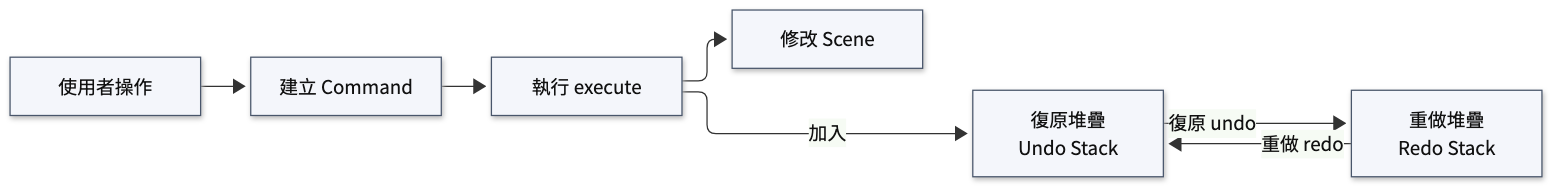
\includegraphics[width=.92\textwidth]{docs/figures/command-history.png}
    \caption{Command、復原與重做的資料流}
    \label{fig:command-history}
\end{figure}

\subsection{Rendering Pipeline}
\label{sec:rendering-pipeline}

Window 開始重繪時，Element tree 會按照各自的局部座標依序 render。輪到 Canvas 之後，CanvasRenderer 先畫 Grid，再按照 Scene 中的順序畫出物件，最後補上工具的 draft overlay。SceneRenderer 會判斷物件是 Shape 還是 Text，再交給對應的 Renderer 呼叫 OpenGL。整條 Rendering Pipeline 如圖~\ref{fig:render-pipeline} 所示。

\begin{figure}[H]
    \centering
    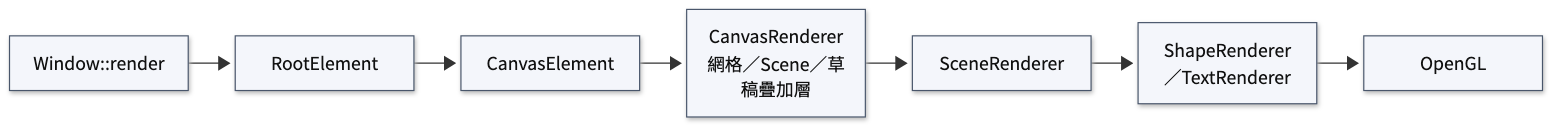
\includegraphics[width=.98\textwidth]{docs/figures/render-pipeline.png}
    \caption{目前的畫面渲染流程}
    \label{fig:render-pipeline}
\end{figure}
